\section{OUT - Data Output}

\subsection{Keyword}

\begin{verbatim}
#OUTPUT_EX
\end{verbatim}

\subsection{Methods}

\begin{table}[h]
%\caption{}
\begin{tabular}{|l|l|l|l|}
\hline
M & S & Subject & Format
\\
\hline
\hline
0 & ? & Contours: all node quantities at defined time interval & RFO
\\
1 & OK & Time curve: all node quantities at given node defined by coordinates (x,y,z) &
\\
2 & ? & Profiles, all time steps &
\\
3 & ? & Profiles, defined time steps &
\\
4 & ? & Time curve: all node quantities at given node defined by number &
\\
5 & OK & Profiles: X-Y plots of specified quantities at given time points & PLT
\\
6 & ? & Profiles: X-Y plots of specified quantities for all time points & PLT
\\
7 & ? & Contours: specified quantities at given time points & PLT
\\
15 & OK & Profiles: along polyline & PLT
\\
\hline
\end{tabular}
\end{table}
M - method, S - status
\normalsize


\subsection{Examples}

\hrule
Method 0
\small
\begin{verbatim}
Contour plots at given time intervals
#OUTPUT_EX
 0 ; method
 1e5 ; output time interval
\end{verbatim}
\normalsize

\hrule
Method 1
\small
\begin{verbatim}
Time curve of all quantities at node given by coordinates
#OUTPUT_EX
 1 ; method
 file.plt ; name of output file
 1.000000e+001  0.000000e+000  0.000000e+000 ; node geometry
\end{verbatim}
\normalsize

\hrule
Method 5
\small
\begin{verbatim}
Profiles: X-Y plots of specified quantities at given time points
#OUTPUT_EX
 5 ; method
 file.plt ; name of output file
 7 ; number of output times
   1.0e+3 1.0e+4 2.0e+4 4.0e+4 6.0e+4 8.0e+4 1.0e+5 ; output times
   10. ; time radius
 4 ; number of output values
   X  PRESSURE1 SATURATION2 TEMPERATURE1 ; names of output values
\end{verbatim}
\normalsize

\hrule
Method 6
\small
\begin{verbatim}
Profiles: X-Y plots of specified quantities for all time points
#OUTPUT_EX
 6 ; method
 file.plt ; name of output file
 4 ; number of output values
   Z   PRESS  HEAD  SATURATION ; names of output values
\end{verbatim}
\normalsize

\hrule
Method 7
\small
\begin{verbatim}
#OUTPUT_EX
 7 ; method:
 file.plt ; name of output file
 1 ; number of output times
   86400. ; output time
   1. ; output time radius
 4 ; number of output values
   X  Y  Z  PRESS ; names of output values
\end{verbatim}
\normalsize

\hrule
Method 10
\small
\begin{verbatim}
#OUTPUT_EX
; Beispiel fuer Ausgabe von Knotendaten in verschiedenen Materialgruppen
10 ; method
 file.plt ; name of output file
  1 1 2 ; mode method data_output_method time
  8.64e+8 ; output time
  1.0 ; output time radius
 5 ; number of output values
   Z  PRESS CONC_1 CONC_2  CONC_3 ; names of output values
\end{verbatim}
\normalsize

\hrule
Method 15
\small
\begin{verbatim}
RFD file:
#OUTPUT_EX
; Profile along polyline
15 ; method
 file.plt ; name of output file
 POLYLINE1 ; polyline name

RFM file with polyline data:
#POLYLINE
POLYLINE1
2 ; number of polyline points
2 ; polyline type
0.0 0.0 0.0 0.000000e+000 5.000000e+002
0.0 6.0 0.0 0.000000e+000 5.000000e+002
0.000000e+000 ; epsilon
1 ; closed
\end{verbatim}
\normalsize

\hrule


\begin{figure}[htb!]
\begin{center}
\footnotesize
\vspace{-0.2cm}
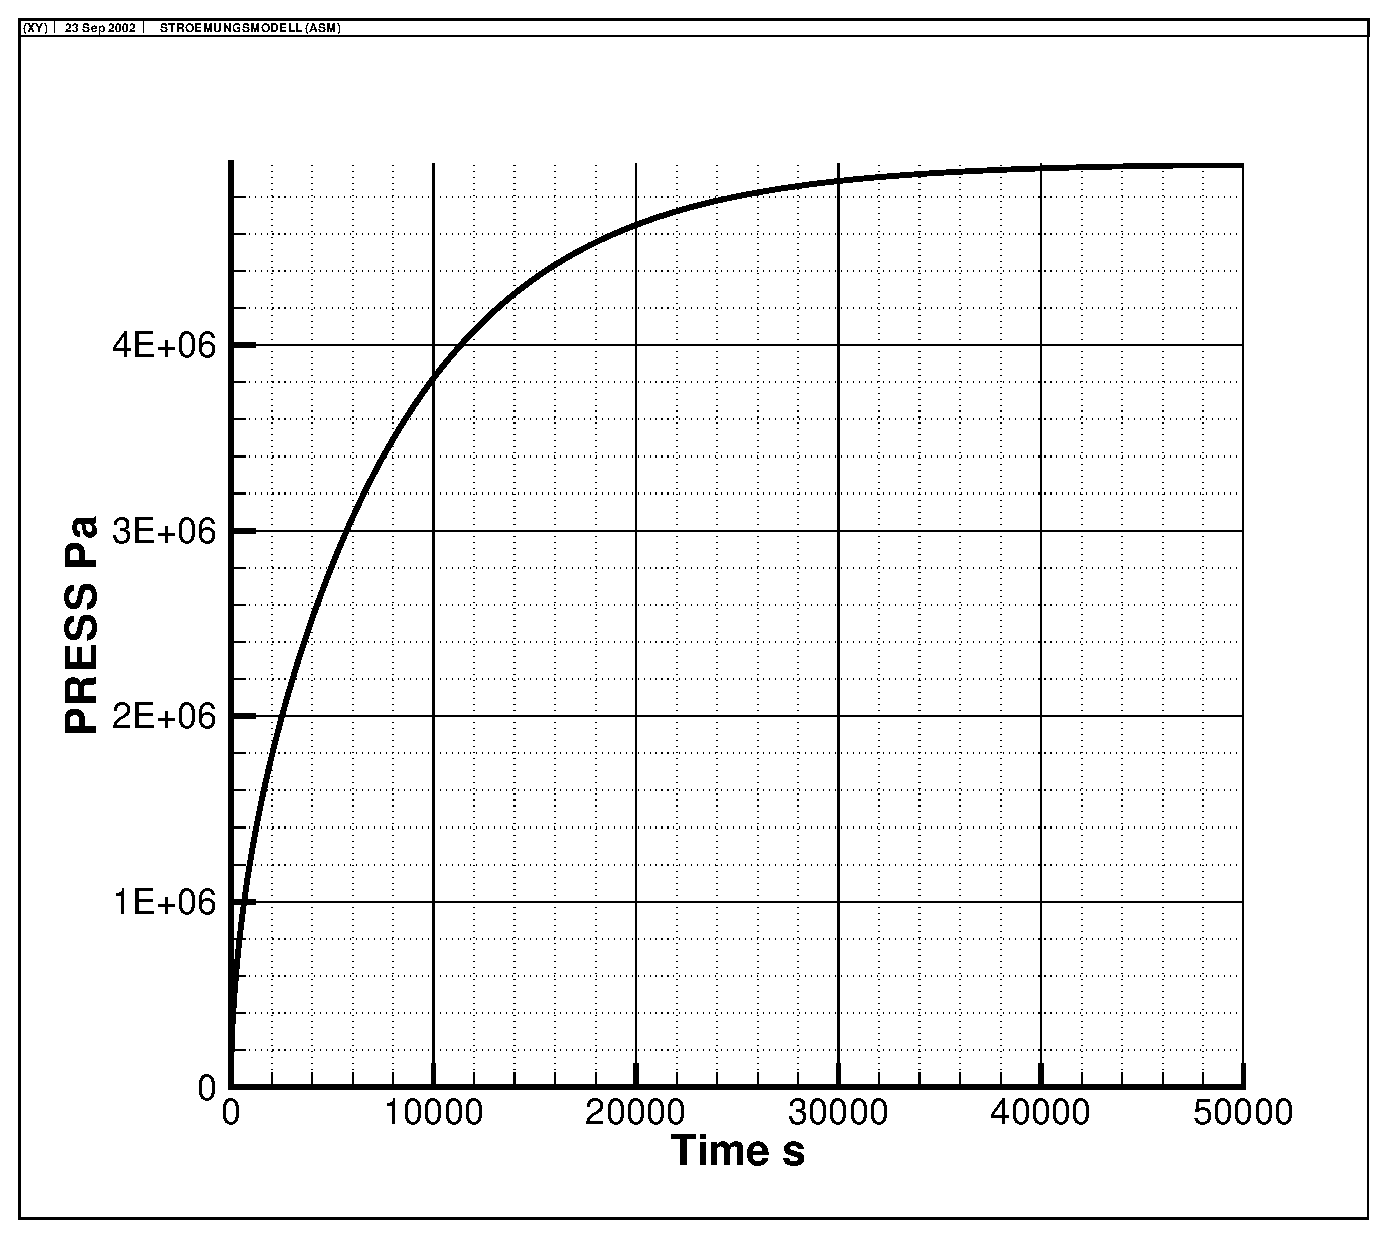
\includegraphics[width=0.5\columnwidth]{figures/out_method1.eps}  % Filename.eps
\caption{
OUT method 1: Time curve of all quantities at node given by coordinates
}
%\label{}
\end{center}
\end{figure}

\begin{figure}[htb!]
\begin{center}
\footnotesize
\vspace{-0.2cm}
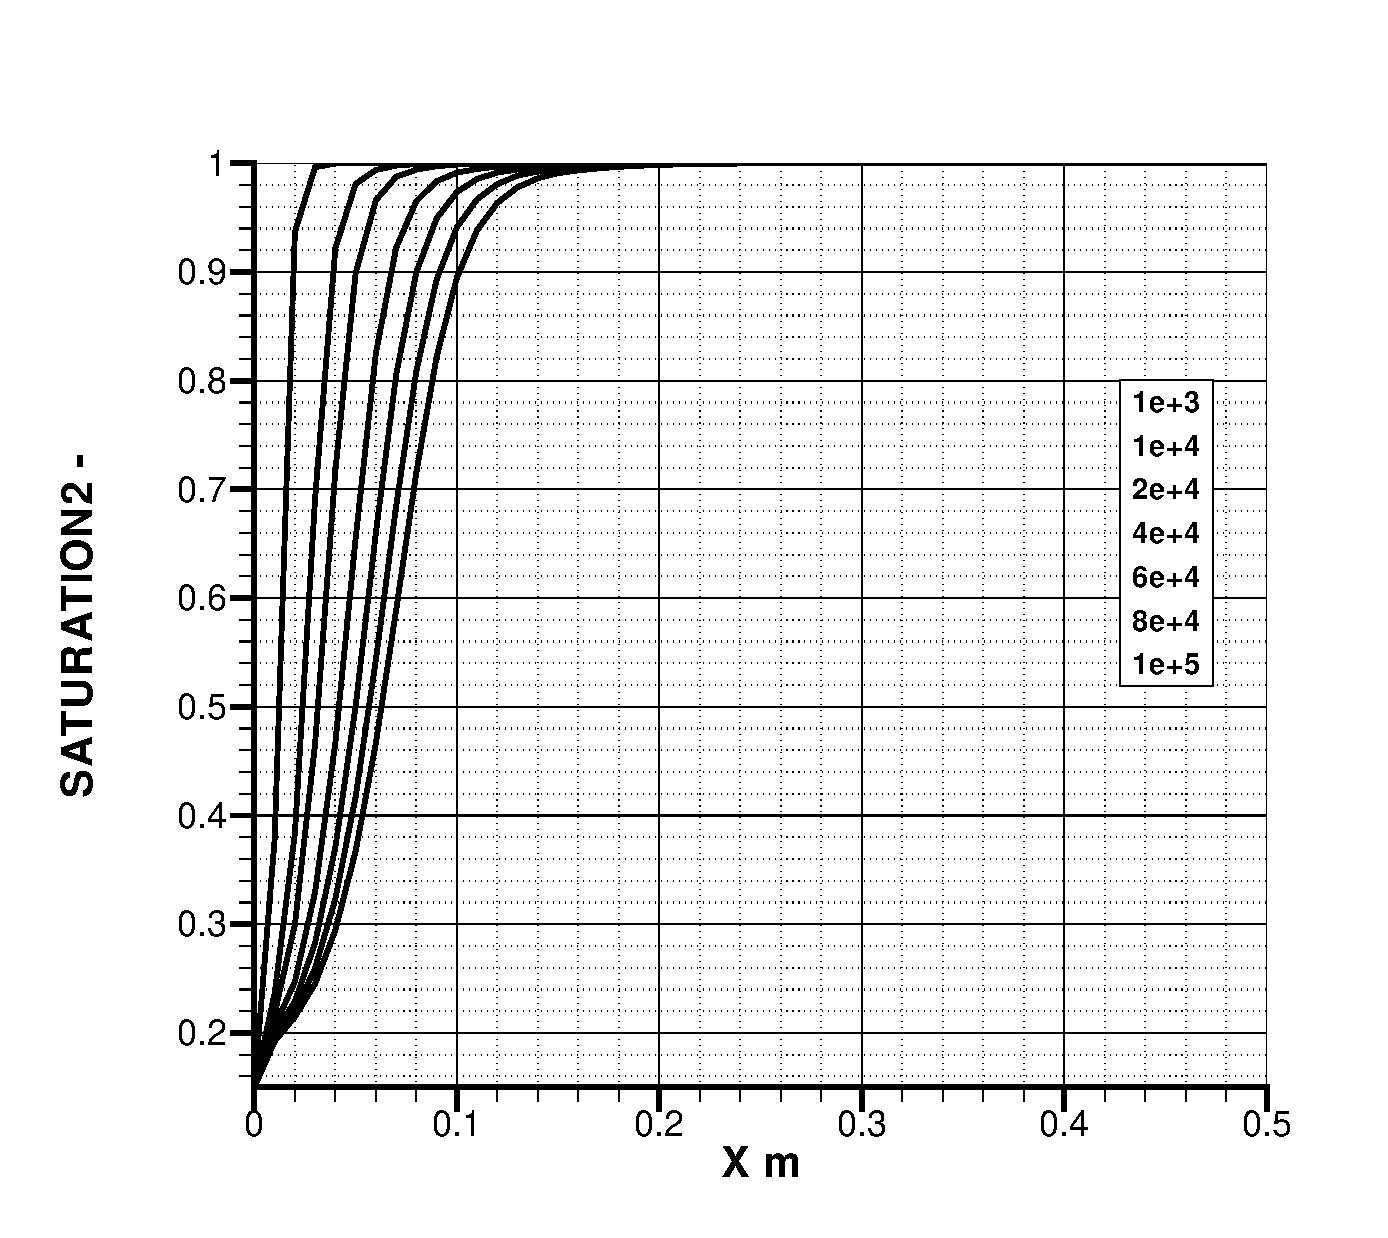
\includegraphics[width=0.5\columnwidth]{figures/out_method5.eps}  % Filename.eps
\caption{
OUT method 5: X-Y plots of specified quantities at given time points
}
%\label{}
\end{center}
\end{figure}

\begin{figure}[htb!]
\begin{center}
\footnotesize
\vspace{-0.2cm}
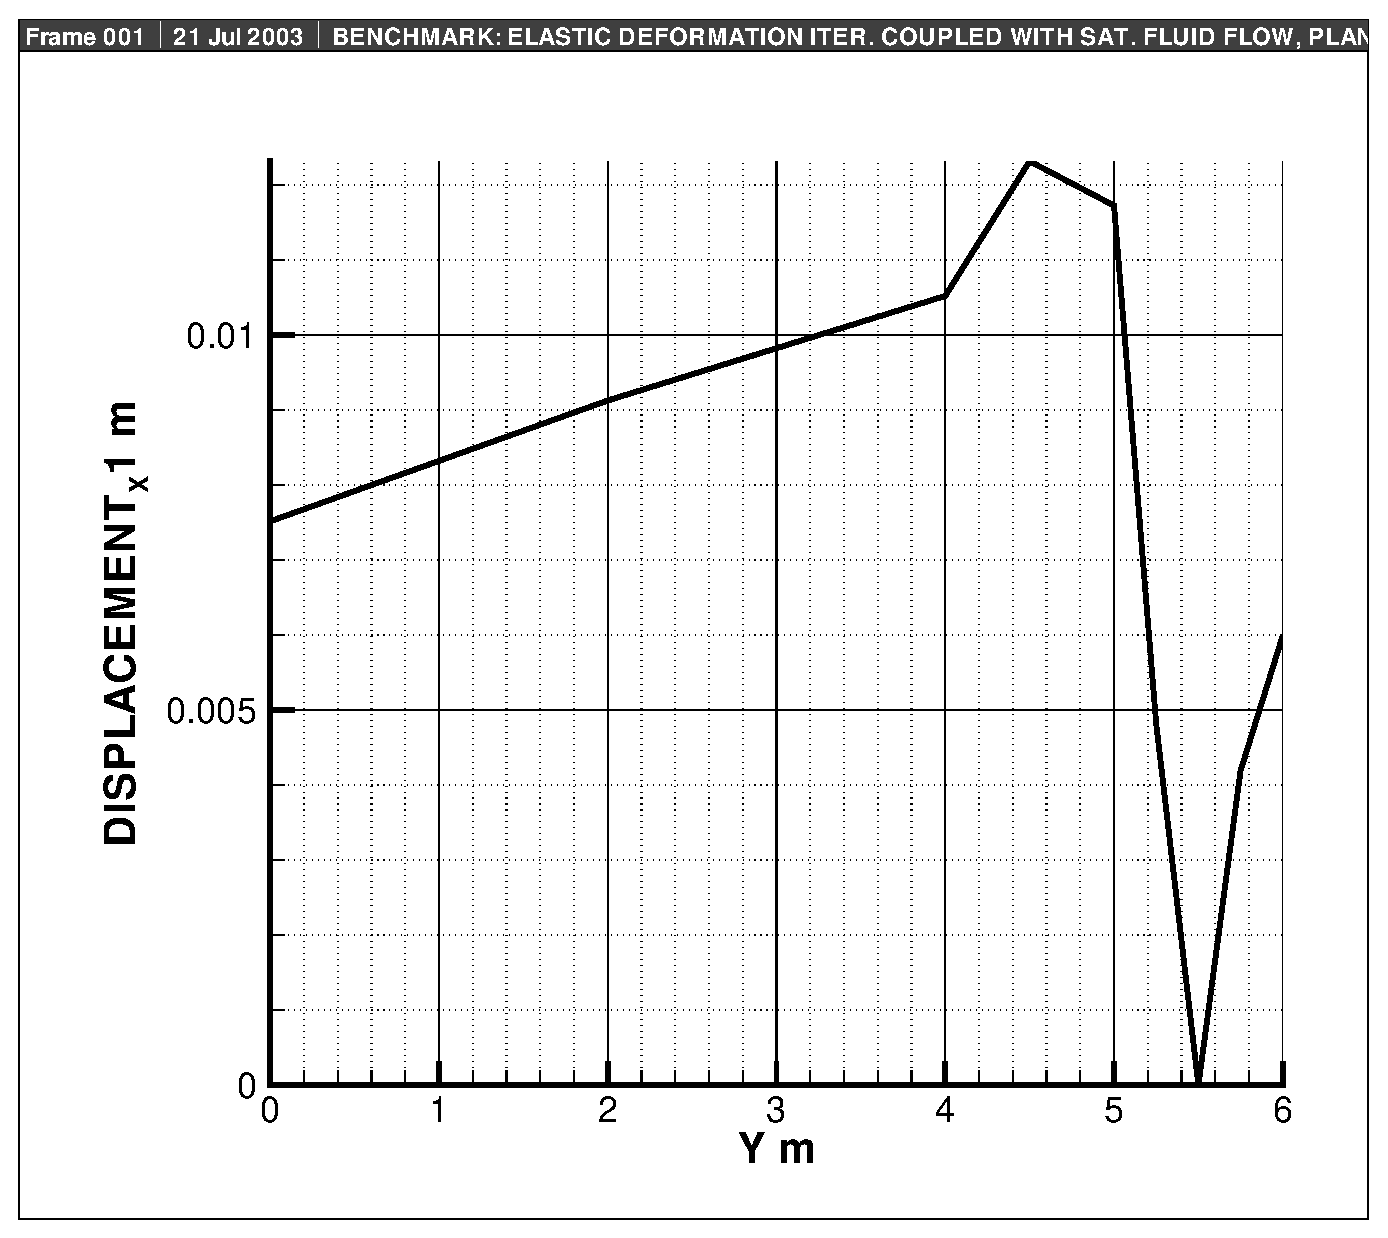
\includegraphics[width=0.5\columnwidth]{figures/out_method15.eps}  % Filename.eps
\caption{
OUT method 15: X-Y plot of specified quantities at given time point along a polyline
(profile along polyline)
}
%\label{}
\end{center}
\end{figure}


\vfill
\LastModified{OK 21.07.2003}
